\subsection{Membrane-magnet system}
\label{sec: Membrane-magnet_system}

The magnet needs to be suspended to allow it to move freely only on the z-axis, to achieve this we need a structure that constrains the lateral motion of the magnet and needs to also be able to vibrate freely with it.
To do this we can use a flexible membrane that can deform under the magnetic field generated by the coil and the magnet. 

As an example, we will analyze the membrane structure of the last type of prototype we implemented %\ref{sec:Flexible_Mat_Prototypes}
\begin{figure}
    \centering
    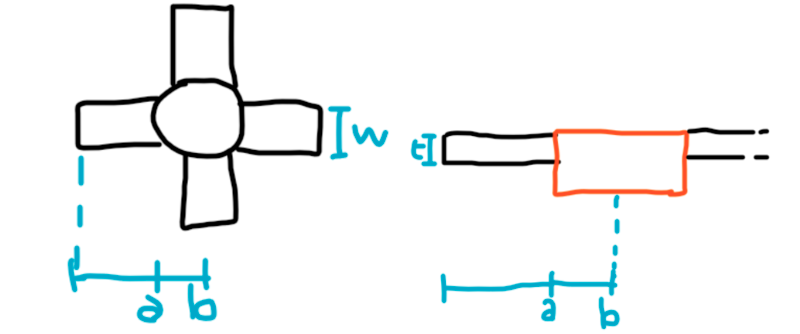
\includegraphics[scale=0.4]{Chapters/Chapter2/Modelling_of_Entire_System/Figures/membrane.png} % TODO: Change image with svg
    \caption[Membrane structure]{Membrane structure of the last prototype.}
    \label{fig:Membrane_structure}
\end{figure}

This membrane is a simple Celtic-cross structure made of thin silicone integrated with the entire structure of the device, the membrane is built with a central cylindrical chamber used to trap the magnet in the center of the cross.
\begin{figure}
    \centering
    \resizebox{.9\linewidth}{!}{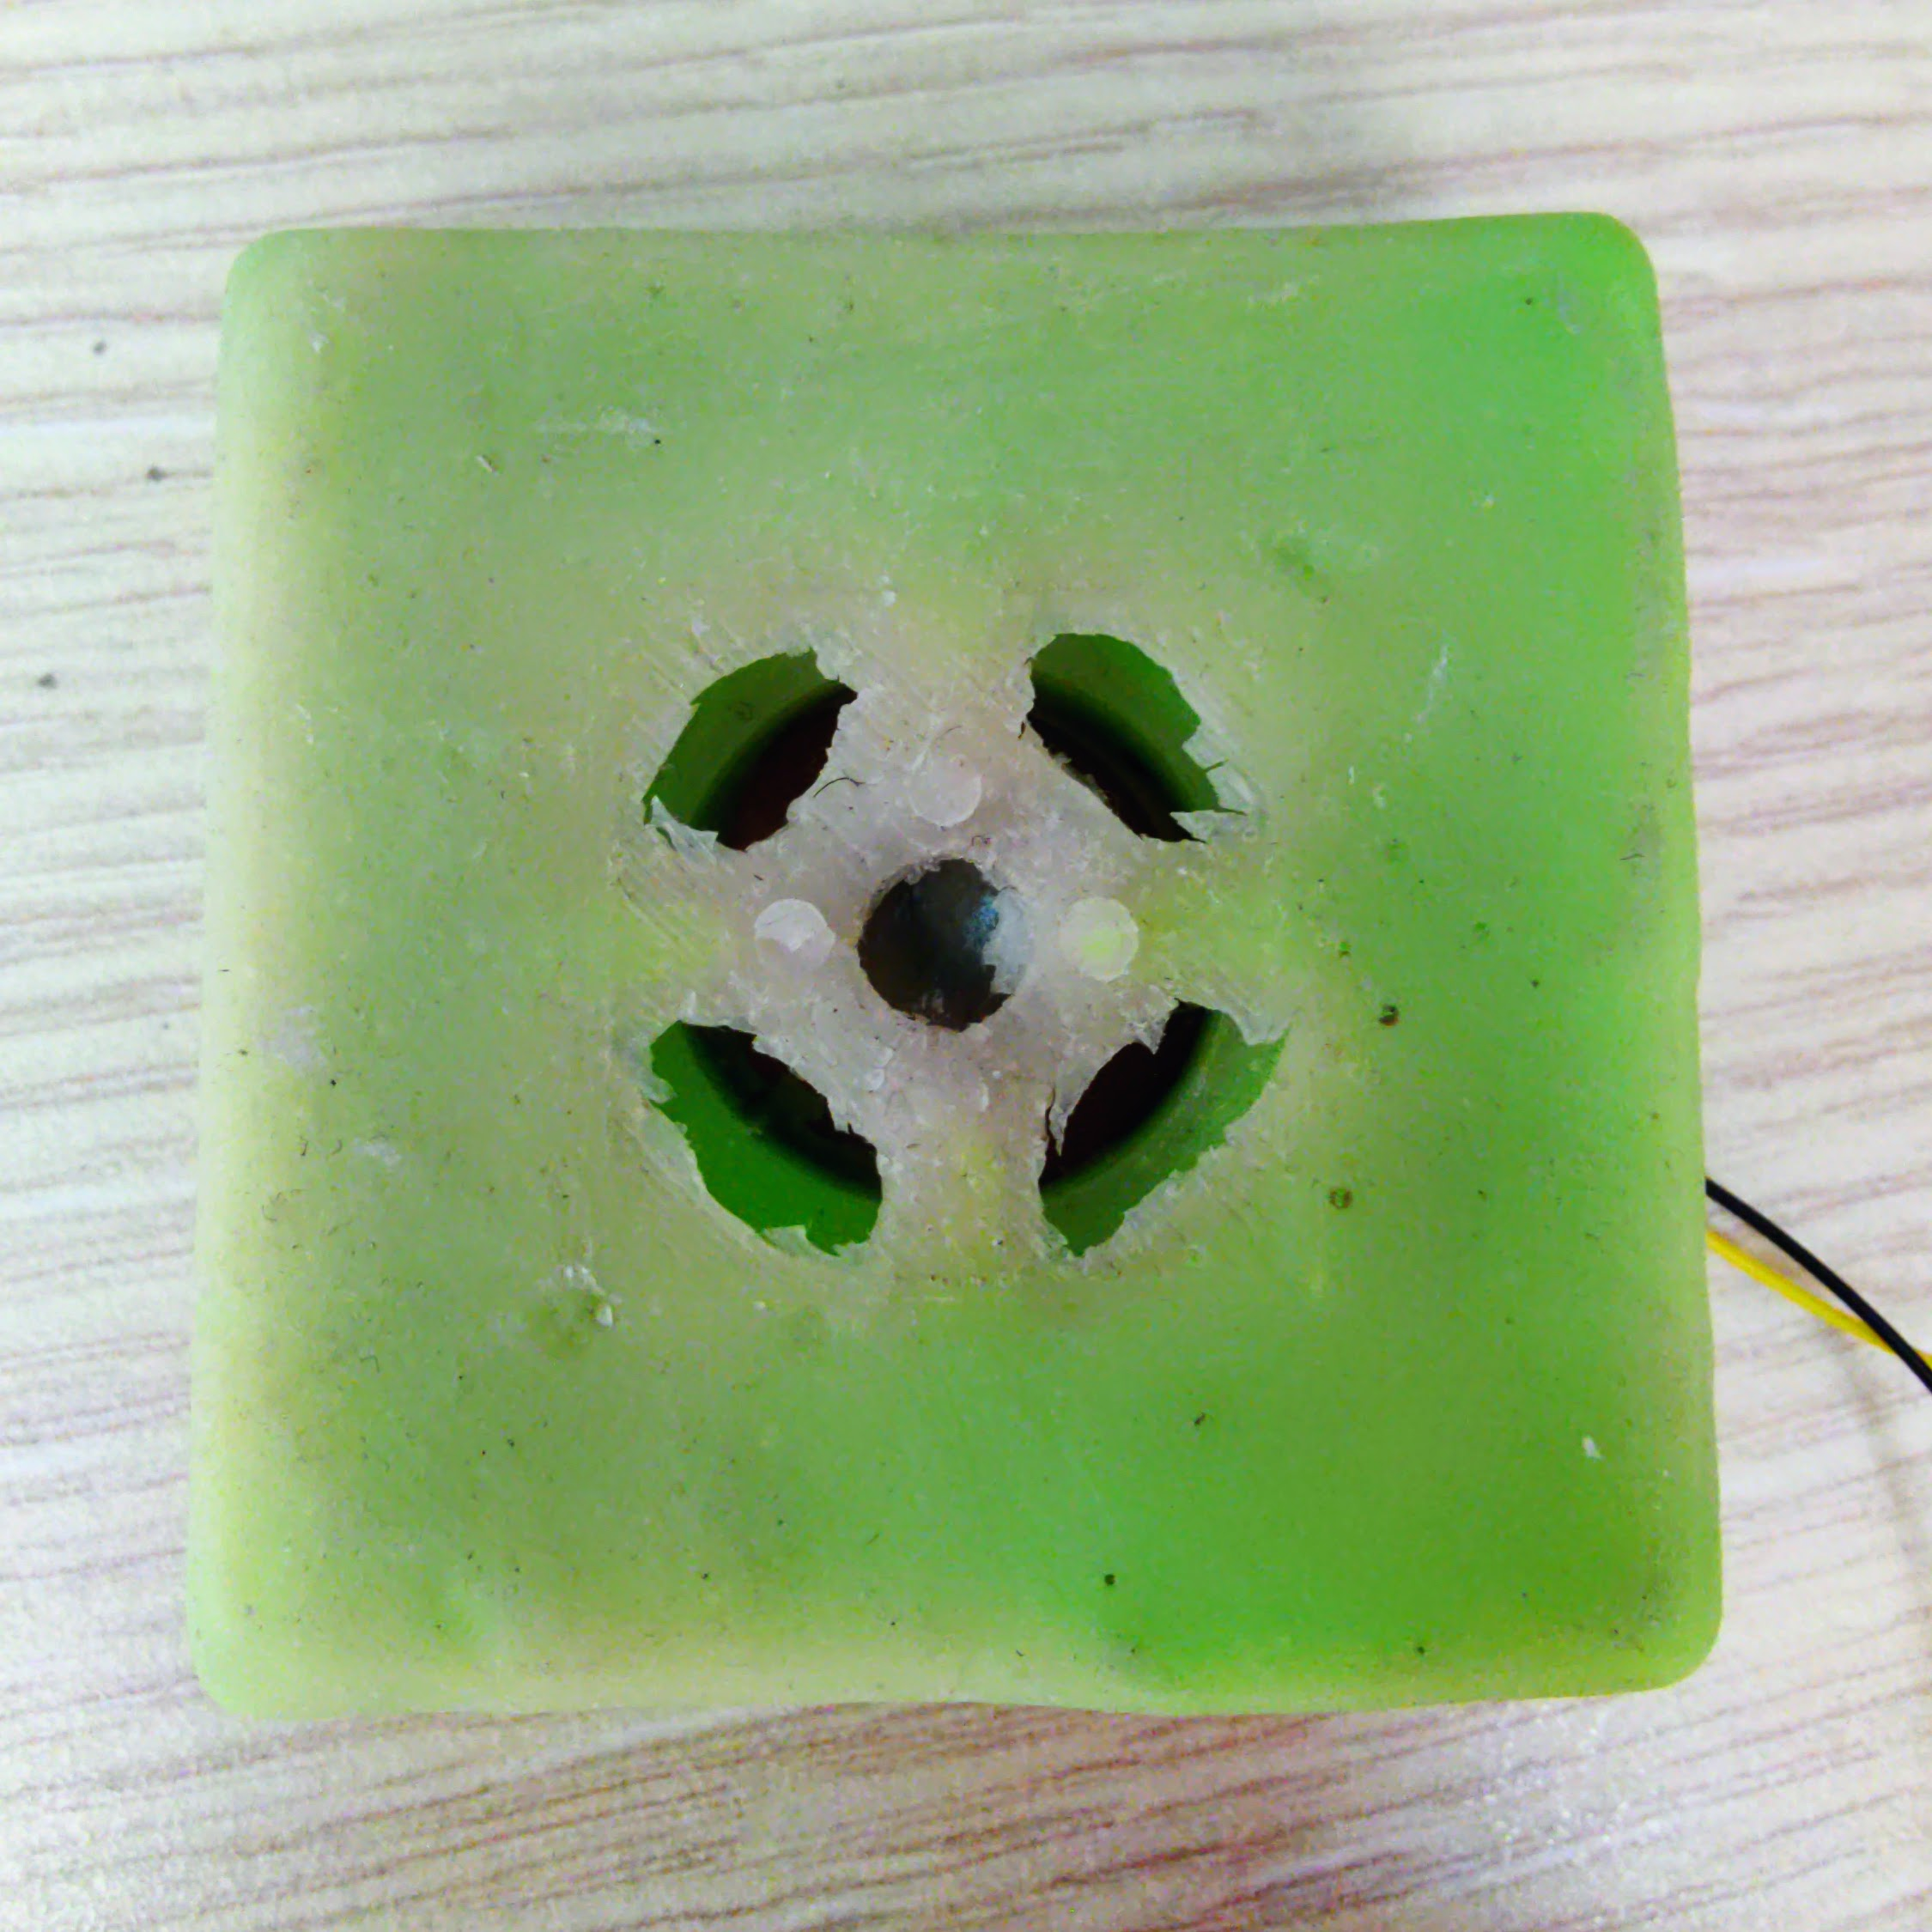
\includegraphics{Chapters/Chapter2/Modelling_of_Entire_System/Figures/Flexible_mat_small_top.jpg}}
    \caption[Membrane mat]{Membrane of the last prototype with the magnet trapped in the center.}
    \label{fig:Membrane_trap}
\end{figure}

The membrane can be modeled as a mass-spring-damper system.
\begin{figure}
    \centering
    \resizebox{.9\linewidth}{!}{
        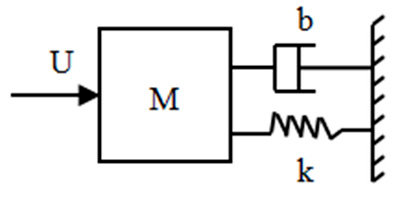
\includegraphics[scale = 0.6]{Chapters/Chapter2/Modelling_of_Entire_System/Figures/membrane_mech_model.png}
        \begin{tikzpicture}
    \begin{scope}[every node/.style={bgelement}]
    \node (start) at (0,0) {};
    \node[right=1 of start] (w) {1: Mech};
    \node[above=1 of w] (Cm) {C: $\frac{1}{ks_{membr}}$};
    \node[below=1 of w] (Rm) {R: b\textsubscript{membr}};
    \node[right=1 of w] (Im) {I: M\textsubscript{magnet}};
    \end{scope}
    \draw[bonds]
    (start) edge [e_in, flow={i}, effort={V}] (w)
    (w) edge [e_out] (Cm)
    (w) edge [e_in] (Rm)
    (w) edge [e_in] (Im);
\end{tikzpicture}    
    }
    \caption{Bond graph of the membrane-magnet system.}
    \label{fig:Membrane_bond_graph}
\end{figure}

\subsubsection{Membrane stiffness}
\label{sec: Membrane_stiffness}
The membrane stiffness can be calculated using Young's modulus of the material, the geometry of the membrane and the load characteristics.

The geometry of the membrane can be modeled as two \textbf{fixed beams} perpendicular to each other and connected at the center.
They are both under a shared \textbf{partially distributed load}, the magnet's weight.
\begin{figure}
    \centering
    \resizebox{0.9\textwidth}{!}{
        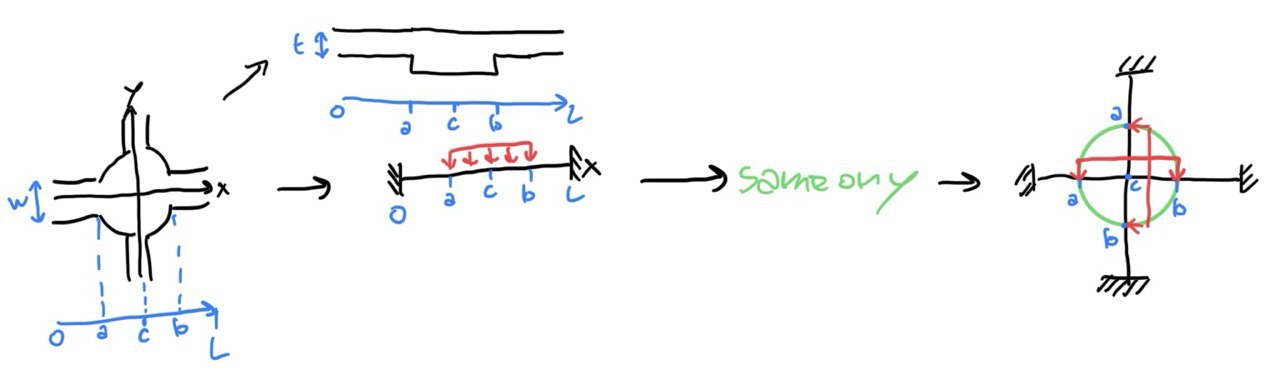
\includegraphics{Chapters/Chapter2/Modelling_of_Entire_System/Figures/membrane_mech_model_v2.jpg} % TODO: Change image with svg
    }
    \caption{Membrane structure simplified as two fixed beams.}
    \label{fig: Membrane_structure_simplified}
\end{figure}

Where we approximate the distribution of weight on the membrane as the weight of the magnet distributed across its diameter.
For each beam, the distributed load can be calculated as:
\begin{equation}
    w = \frac{\frac{M_{magnet}}{2} g}{2 r}
\end{equation}
Where:
\begin{itemize}
    \item $w$ is the distributed load [N/m]
    \item $M_magnet$ is the mass of the magnet [N]
    \item $g$ is the gravitational acceleration [m/s\textsuperscript{2}]
    \item $r$ is the radius of the magnet [m]
\end{itemize}

We approximate by considering only half of the magnet's weight as we have two beams supporting the magnet.

Then the stiffness of a single beam is defined as:
\begin{equation}
    ks = \frac{P}{\delta_{max}}
\end{equation}
Where:
\begin{itemize}
    \item $ks$ is the stiffness of the beam [N/m]
    \item $P$ is the load on the beam [N]
    \item $\delta_{max}$ is the deflection of the beam [m]
\end{itemize}

Considering the structure shown in figure \ref{fig: Membrane_structure_simplified}, the maximum deflection of a fixed beam under a distributed load can be calculated as:
\begin{equation}
    \label{eq: Beam_deflection}
    \delta_{max} = -\frac{R_A c^3}{6 E I} - \frac{M_A c^2}{2EI} + \frac{w (c-a)^4}{24 EI}
\end{equation}
Where:
\begin{itemize}
    \item $\delta$ is the deflection of the beam [m]
    \item $R_A$ is the reaction force at the origin of the beam [N]
    \item $M_A$ is the moment at the origin of the beam [Nm]
    \item $E$ is the Young's modulus of the material [Pa]
    \item $I$ is the second moment of inertia of the beam [m\textsuperscript{4}]
    \item $w$ is the distributed load [N/m]
    \item $c$ is the distance between the origin of the beam and its center [m]
    \item $a$ is the distance between the origin of the beam and the start of the distributed load [m]
\end{itemize}
We will only focus on the calculation of the second moment of inertia of the beam, the equations for the other parameters can be found in the reference \cite{statics_fixed_beam}.

The beam can be simplified as a parallelepiped with a rectangular section, and the second moment of inertia on x can be calculated as:
\begin{equation}
    \label{eq: Beam_inertia}
    I_x = \frac{w t^3}{12}
\end{equation}
Where:
\begin{itemize}
    \item $I_x$ is the second moment of inertia on the x-axis [m\textsuperscript{4}]
    \item $w$ is the width of one membrane arm as in figure \ref{fig: Membrane_structure_simplified}[m]
    \item $t$ is the thickness of the membrane as in figure \ref{fig: Membrane_structure_simplified}[m]
\end{itemize}

Then we can consider the 2 beams as 2 springs in parallel, the total stiffness of the membrane can be calculated as:
\begin{equation}
    ks_{membr} = 2 ks
\end{equation}


\subsubsection{Membrane damping}
The damping for a cantilever beam is neglectable, so we can remove the resistive component from the mechanical model.
\begin{figure}
    \centering
    \resizebox{.9\linewidth}{!}{
        \begin{tikzpicture}
    \begin{scope}[every node/.style={bgelement}]
    \node (start) at (0,0) {};
    \node[right=1 of start] (w) {1: Mech};
    \node[above=1 of w] (Cm) {C: $\frac{1}{ks_{membr}}$};
    \node[right=1 of w] (Im) {I: M\textsubscript{magnet}};
    \end{scope}
    \draw[bonds]
    (start) edge [e_in, flow={i}, effort={V}] (w)
    (w) edge [e_out] (Cm)
    (w) edge [e_in] (Im);
\end{tikzpicture}    
    }
    \caption{Final mechanical bond-graph of the membrane and magnet.}
    \label{fig:Membrane_bond graph_without_damping}
\end{figure}

